\documentclass[conference]{IEEEtran}
\usepackage[utf8]{inputenc}
\IEEEoverridecommandlockouts
% The preceding line is only needed to identify funding in the first footnote. If that is unneeded, please comment it out.
\usepackage{cite}
\usepackage{amsmath,amssymb,amsfonts}
\usepackage{algorithmic}
\usepackage{graphicx}
\usepackage{textcomp}
\usepackage{xcolor}
\usepackage{url}
\def\BibTeX{{\rm B\kern-.05em{\sc i\kern-.025em b}\kern-.08em
    T\kern-.1667em\lower.7ex\hbox{E}\kern-.125emX}}
\begin{document}

\title{Deep Learning for Public Health: Predicting Obesity with Neural Networks\\
{\footnotesize \textsuperscript}
\thanks{}
}

\author{
    \begin{tabular}{cc}
        \begin{tabular}{@{}c@{}}
            1\textsuperscript{st} Jairus Legion \\
            \textit{California State Polytechnic University, Pomona} \\
            \textit{Computer Science} \\
            Pomona, CA \\
            jmlegion@cpp.edu
        \end{tabular}
        &
        \begin{tabular}{@{}c@{}}
            2\textsuperscript{nd} Mayela Ancheta \\
            \textit{California State Polytechnic University, Pomona} \\
            \textit{Computer Science} \\
            Pomona, CA \\
            mancheta@cpp.edu
        \end{tabular}
        \\
        \\
        \begin{tabular}{@{}c@{}}
            3\textsuperscript{rd} Jessica Pinto \\
            \textit{California State Polytechnic University, Pomona} \\
            \textit{Computer Science} \\
            Pomona, CA \\
            jmpinto@cpp.edu
        \end{tabular}
        &
        \begin{tabular}{@{}c@{}}
            4\textsuperscript{th} Anh Tu Nguyen \\
            \textit{California State Polytechnic University, Pomona} \\
            \textit{Computer Science} \\
            Pomona, CA \\
             tunguyen@cpp.edu
        \end{tabular}
        \\
        \\
        \begin{tabular}{@{}c@{}}
            5\textsuperscript{th} Moller Myint \\
            \textit{California State Polytechnic University, Pomona} \\
            \textit{Computer Science} \\
            Pomona, CA \\
            mamyint@cpp.edu
        \end{tabular}
        &
        \begin{tabular}{@{}c@{}}
            6\textsuperscript{th} Alison Ching \\
            \textit{California State Polytechnic University, Pomona} \\
            \textit{Computer Science} \\
            Pomona, CA \\
            aching@cpp.edu
        \end{tabular}
    \end{tabular}
}



\maketitle

\begin{abstract}
Obesity is a growing health concern worldwide, highlighting an increasingly crucial need for better tools to understand and predict its root causes. Traditional methods, such as analyzing body mass index (BMI) by itself, often overlook the underlying attributes linked to obesity and lead to generalized diagnoses. In this project, we used a publicly available obesity prediction dataset to develop a machine learning model capable of classifying individuals across seven distinct obesity levels. The dataset includes 2,111 samples, 17 attributes related to diet, physical activity, alcohol consumption, technology use, and transportation habits, and 1 column for the final class. We enhanced this dataset by engineering an additional feature, BMI, and implemented Principal Component Analysis (PCA) to explore dimensionality reduction in order to efficiently and effectively predict the level of obesity for an individual.
Our model was built using an artificial neural network (ANN) to perform multi-class classification. We split the data into a training, validation, and testing set. The model was evaluated using accuracy, F1-score, and the Brier score to ensure both predictive performance and proper calibration are optimized. Experimental results confirmed that the Multi-Layer Perceptron significantly outperformed the linear Perceptron, particularly with a high and complex separation of classes. Visualizations using PCA and t-SNE revealed distinct class clustering after the model predictions, reinforcing the ANN’s classification strength. Our findings show how including diverse lifestyle data, rather than relying solely on BMI, can lead to more precise and meaningful obesity classifications, supporting early intervention and better-targeted public health efforts.

\end{abstract}

\section{Introduction}
Obesity has emerged as one of the most pressing public health challenges of the 21st century, with rates steadily increasing worldwide. As it is closely associated with chronic conditions such as heart disease, diabetes, and certain cancers, early detection and prevention have become critical to managing long-term health issues. As mentioned before, it is imperative to analyze deeper causes of the illness than a patient’s BMI in order to provide appropriate care for their diagnosis and encourage them to make improvements in their lifestyles.
Machine learning provides an innovative approach to tackling this matter by leveraging complex data to uncover hidden patterns and make informed predictions. In this project, we aim to develop a predictive model that classifies individuals into specific obesity categories based on their lifestyle and behavioral factors. Our goal is to build a model that not only performs well on existing data but also accurately predicts classifications for unseen individuals with diverse habits and conditions. 
We utilize the publicly available Obesity Prediction Dataset, which contains detailed self-reported data from individuals across various countries. This dataset includes a wide range of attributes–from dietary habits and physical activity to technology usage and transportation modes–that influence obesity levels. By applying an artificial neural network (ANN) and evaluating its performance through rigorous metrics like the F1-score and Brier score, we seek to demonstrate how machine learning can aid in healthcare decision-making and obesity prevention efforts.
Through this research, we aim to contribute to the growing body of work that applies artificial intelligence to public health, providing insights that are not only statistically significant but also clinically meaningful.




\section{Dataset}



The dataset used is an Obesity Prediction Dataset available from the UCI Machine Learning Repository that provides different lifestyle factors to relate to obesity levels, ranging from Insufficient Weight to Obesity III. This dataset predicts obesity levels in individuals residing in Mexico, Peru, and Colombia. Our team has acquired this dataset through Kaggle, a public database platform that provides detailed information about each dataset provided. Most of the data has been generated using synthetic techniques in tandem with responses from users through a web platform. The dataset is in CSV format and contains 17 attributes and 2111 samples in total. Table 3.1 below shows all the attributes and what each of them mean.
\begin{figure}[htbp]
\centering
\includegraphics[width=0.45\textwidth]{cs4210attributes.png}
\caption{Table 3.1}
\label{Table 3.1}
\end{figure}

In addition to the original 17 attributes, we introduced an 18th feature, Body Mass Index (BMI). The values within the column were calculated using the standard medical formula, weight divided by height square (kg/m²) to provide a numerically interpretable value of physical health. While the dataset already included height and weight values, the BMI column offers an overall view of body composition and is widely used in clinical and public health settings. Including BMI allowed us to explore how using this calculated metric compares to using simply height and weight values in terms of its impact on classification accuracy.

Prior to running the model, we also made sure to analyze the Obesity Dataset and search for notable characteristics that may affect our model’s performance. To do this, we utilized a combination of bar charts, box plots, and stacked bar charts—each selected to illuminate a distinct aspect of the data. A bar chart of class frequencies, seen in Figure 3.1 provides a rapid assessment of target‐variable balance, which is critical for identifying potential sampling or class-weighting strategies before model training. Our visualization shows that we have a relatively even distribution of classes within our dataset, allowing us to skip upsampling or downsampling to mitigate the risks of class imbalance.

\begin{figure}[htbp]
\centering
\includegraphics[width=0.45\textwidth]{ObesityDist.png}
\caption{Shows the distribution of classes in our dataset. }
\label{Table 3.1}
\end{figure}

\begin{figure}[htbp]
\centering
\includegraphics[width=0.45\textwidth]{fig3.2.png}
\caption{Stacked Bar Chart for family history with overweight attribute}
\label{Table 3.1}
\centering
\includegraphics[width=0.45\textwidth]{fig3.3.png}
\caption{Weight By Obesity Class Boxplot}
\label{Table 3.1}
\end{figure}

Stacked bar charts, such as the one in Figure 3 for categorical predictors (Gender, family history, transport mode, etc.) expose how each category partitions into obesity classes, directly revealing which demographic or behavioral subgroups are most associated with different obesity levels. Finally, box plots, illustrated in Figure 4 are ideal for comparing continuous features (Age, Weight, FCVC, etc.) across classes: by visualizing medians, quartiles, and outliers side-by-side, we can discern whether, for example, heavier obesity categories truly exhibit consistently higher weights or if substantial overlap exists that might confound classification.

We see Figure 3 and Figure 4 play a particularly important role in this. First, the stacked bar chart of Obesity Classes by Family History in Figure 3 shows that individuals reporting a family history of overweight display a markedly larger share of overweight and obese categories than those without such history, underscoring genetic predisposition as a key categorical predictor. Second, Figure 4 shows the Weight by Obesity Class box plot which demonstrates a clear, monotonic increase in median weight from ``Normal\_Weight'' through ``Obesity\_Type\_III,'' with interquartile ranges that separate progressively—confirming weight as a highly discriminative numerical feature. Together, these targeted plots not only validate our feature-selection choices but also guide subsequent model design by highlighting where class separation is strongest.

\begin{figure}[htbp]
\centering
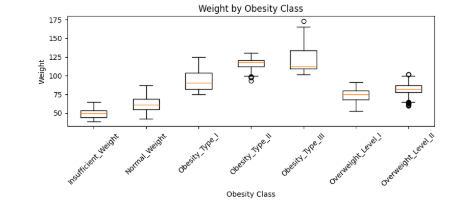
\includegraphics[width=0.45\textwidth]{fig4.png}
\caption{Shows family history of being overweight distributed over height }
\label{Table 3.1}
\end{figure}

Although calculating obesity is our primary goal, seeing how important attributes are distributed amongst one another can be useful in detecting trends in the data that may not be so obviously connected to the direct classification of obesity levels. Height and family\_history\_with\_overweight were both attributes that reached within the top 5 of our model which we will discuss more about later in Section 4. Thus, Figure 5 above displays family history of being overweight distributed over height. From this, we see that although category 2 for height has the most samples, the overall data shows that those who are in category 3, a.k.a. those who are the tallest, have the highest ratio of people with a family history of obesity. This insight suggests that even among individuals with height above average (a trait often associated with leanness), genetic predisposition still has the potential to have a large impact in obesity risk. Identifying such relationships enable us to uncover hidden dependencies between physical traits and heredity factors that influence obesity. Equipped with this knowledge, we can make our model more precise in its predictions and ultimately, improve its accuracy. This contributes to our goal of creating a more detailed and personalized obesity risk assessment that extends beyond the standard BMI metric and incorporates deeper patterns found in the data. 

\section{Methodology}
\subsection{Preprocessing}
As specified in Section 3, our dataset is made up of 16 attributes, all of which are utilized by the artificial neural network to learn intricate details, patterns, and relationships within the data. Despite the benefits of having many attributes for training, having an excess number of attributes that do not contribute significantly to predictions may lead to overfitting, increased computational costs, and difficulty in generalization. Considering the downfalls of having too many irrelevant features, we tested the performance of our model using dimensionality reduction with the Principal Component Analysis (PCA). Using all the attributes in the original dataset and not utilizing the results of PCA, we received an accuracy of 62.6\% with the perceptron model and 86.7\% with the multi-layer perceptron model. Here is where we began to see that the multi-layer perceptron performs considerably better than the perceptron, but further results will support this claim in the next section of this paper. 

While an accuracy of 86.7\% is not lacking by any means, our goal was to find a way to improve this result nonetheless. Since there was a chance that one of the 16 features might be introducing noise or redundancy, potentially interfering with the neural network’s ability to learn meaningful patterns, we moved onto our next solution: PCA. We first had to convert our dataset into numeric values, since that is what PCA can operate on rather than categorical string data. After this conversion, we ran PCA with 1 component to capture the direction of maximum variance. This allowed us to evaluate which features had the highest significance and were most influential in the first principal component — guiding our feature selection process. The results of PCA, shown in Table 4.1, helped us identify the most informative features based on their contributions to the first principal component. This guided our feature selection process, allowing us to test both the perceptron and multi-layer perceptron models with various subsets of features. The results of these subset combinations with both the perceptron and multi-layer perceptron models are shown in Figure 6.

\begin{figure}[htbp]
\centering
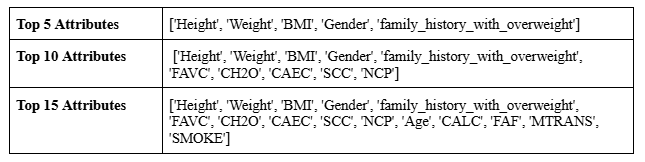
\includegraphics[width=0.45\textwidth]{fig6.png}
\caption{Results of PCA with component = 1}
\label{Table 3.1}
\end{figure}

\subsection{Training and Testing the Model}
In order to accurately train our model and produce the best results, we will disseminate our dataset into three parts: training, testing, and validation. The training set is the largest set and will contain about 80\% of the total samples. The training set will teach the model to identify patterns and make predictions. The testing set will remain untouched during the training process and will only be used once the model has been trained to evaluate how it is performing with new samples. Finally, the validation set is created to be a part of the training process and provide a first initial test with unseen data. It helps to fine tune and optimize the model to help prevent overfitting. A validation set is not required when training a machine learning model, however since we are working with medical data and want to provide realistic and accurate results, we chose to add it to our training process to improve our model. Since our model will not be self-training, all our samples will include the ground truth, which in our case would be the patient’s level of obesity. This prediction will be based on the feature values from 16 different patient attributes listed and expounded in Section 3. Considering that each patient can be categorized into only one of seven different obesity levels, this model will conduct multi-class classification on the data.

\subsection{Chosen Model Specifications}\label{AA}

For this project, we have chosen to use an artificial neural network (ANN), a machine learning model inspired by the human brain’s neural structure. ANNs are made up of layers of artificial neurons, also called perceptrons, which process input data and learn patterns to perform tasks like classification or prediction.

An ANN is composed of multiple perceptrons, and each perceptron is typically structured in layers: an input layer where raw data is taken in, one or more hidden layers where computation occurs, and a final output layer which produces the decision. The operations that perceptrons perform can be defined by the equation:

\[
z = \sum_{i=0}^{n} x_i w_i + b
\]

where:
\begin{itemize}
    \item $n$ = number of input features
    \item $x_i$ = input feature $i$
    \item $w_i$ = corresponding weight
    \item $b$ = bias term
    \item $z$ = weighted sum passed through an activation function
\end{itemize}

ANNs learn through forward propagation, loss computation, and backpropagation. In forward propagation, inputs pass through the network layer by layer, producing an output prediction.

The prediction error is measured using the categorical cross-entropy loss function, given by:

\[
E = -\sum_{i=0}^{n} \sum_{j=0}^{C} t_{ij} \log(o_{ij})
\]

where:
\begin{itemize}
    \item $n$ = number of training samples in the batch
    \item $C$ = number of classes
    \item $t_{ij} = 1$ if sample $i$ belongs to class $j$, otherwise $0$
    \item $o_{ij}$ = predicted probability of class $j$ for sample $i$ (from the softmax output)
\end{itemize}

Backpropagation computes the gradients of the loss with respect to each weight using the chain rule. These gradients guide how to adjust the weights to reduce prediction error.

Weights are updated using gradient descent:

\[
w = w - \eta \frac{\partial L}{\partial w}
\]

where:
\begin{itemize}
    \item $\eta$ = learning rate
    \item $\frac{\partial L}{\partial w}$ = gradient of the loss with respect to the weight
\end{itemize}



\subsection{Machine Learning Model Evaluation}
To ensure that our model is valid and can make accurate predictions with unseen data, we will perform a thorough model evaluation using the test set mentioned in Section 4a. The test set includes samples that make up about 10\% of the original dataset and will remain unused during training and validation stages.  This is to ensure that the evaluation metrics reflect the model’s real-world performance. In order to evaluate the predictive performance of the  model, we will be using mean accuracy and the F1-score. The F1 score is important in the context of an imbalanced dataset as it takes into account both precision and recall, which offers a balanced assessment of the model’s ability to classify both majority and minority obesity levels. This is extremely important in healthcare classification tasks where certain obesity levels are underrepresented in this dataset but clinically significant in real world scenarios.
In addition to the mean accuracy and F1-score, we will also be finding the Brier score to evaluate the calibration of the model’s predicted probabilities. The Brier score is a metric that combines aspects of calibration and discrimination, where lower values indicate superior model performance. It’s important in medical contexts as it penalizes overfitting, which would lead to poor calibration [3].

\section{Results}
Based on the results we received from training and testing both the perceptron and multi-layer perceptron (MLP)  model, we created confusion matrices to show how well the model distinguished between classes and to make it easier to identify misclassifications. The Perceptron Classifier is a linear model suitable for linearly separable data. From Figure 8, the Perceptron Confusion Matrix showed a significant number of misclassifications between adjacent obesity levels, such as Normal\_Weight and Overweight\_Level\_I. This shows that with its limited layers that can perform arithmetic operations, the Perceptron struggles to classify using this dataset. 


\begin{figure}[htbp]
\centering
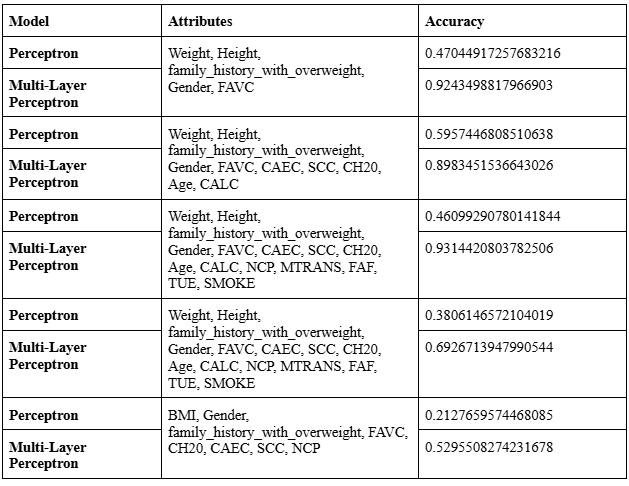
\includegraphics[width=0.45\textwidth]{fig7.png}
\caption{Accuracies using the perceptron and multi-layer perceptron models and ranked PCA attributes}
\label{Table 3.1}
\end{figure}


This supports our results showing that the Multi-Layer Perceptron (MLP), with its more complex architecture and the ability to generate non-linear decision boundaries, had much more success classifying with this dataset.  From Figure 9, it is clear that the MLP Classifier achieved significantly higher accuracy, particularly on clearly separable classes such as Obesity\_Type\_III and Insufficient\_Weight, with fewer off-diagonal errors. High accuracy across most classes are observed, such as Obesity\_Type\_III performing with 65/65 correctness and Obesity\_Type\_I performing with 69/70 correctness. These matrices confirmed that the MLP model was more reliable for multi-class classification in this domain.

\begin{figure}[htbp]
\centering
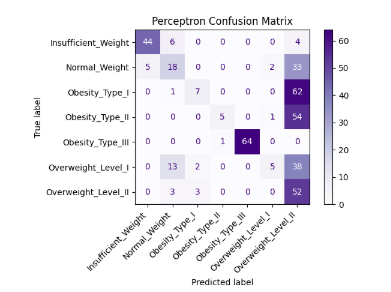
\includegraphics[width=0.45\textwidth]{fig8.png}
\caption{shows the confusion matrix for the Perceptron Classifier.}
\label{Table 3.1}
\end{figure}
\begin{figure}[htbp]
\centering
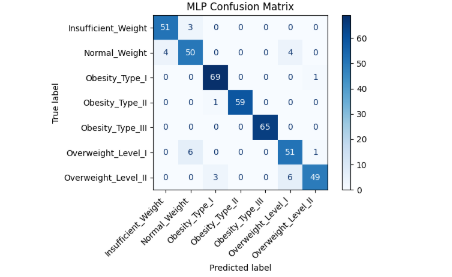
\includegraphics[width=0.45\textwidth]{fig9.png}
\caption{shows the confusion matrix for the MLP Classifier.}
\label{Table 3.1}
\end{figure}

Given the widespread use of Body Mass Index in public health settings, we created an additional attribute in our dataset to represent this. The BMI column was calculated using the height and weight columns provided to us in the original kaggle dataset as mentioned previously in section 3. Our original motive was to analyze whether incorporating BMI as a single input attribute would improve the model’s performance. After testing the model with only the BMI column rather than separate height and weight values, we found the opposite to be true and a significant drop in classification accuracy. From this, it leads to the fact that while BMI may be a comprehensive simplified view of body composition, it has the potential to skew patterns otherwise obvious in the raw height and weight data. As seen in Table 8 above, when the BMI attribute was used to replace the Height and Weight attributes, the accuracy was significantly lower for each model than when the Height and Weight attributes were included. Moreover, we receive accuracies greater than 90\% for all the multi-layer perceptron models regardless of the number of attributes chosen.

\begin{figure}[htbp]
\centering
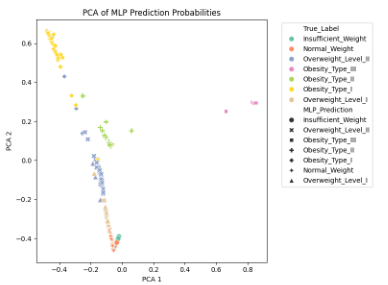
\includegraphics[width=0.45\textwidth]{fig10.png}
\caption{shows the PCA of MLP predicted class probabilities.}
\label{Table 3.1}
\end{figure}

Additionally, the Principal Component Analysis (PCA) was applied to the MLP’s predicted class probabilities to visualize the structure of the classification output in two dimensions. The PCA in Figure 10 helps observe the overall structure of how well the model separates obesity categories. Several obesity classes, especially the extremes, formed distinct clusters, validating the MLP’s ability to differentiate them. Some overlap was observed between mid-range categories such as between Normal\_Weight, Overweight\_Level\_I, and Overweight\_Level\_II, reflecting similarity in their feature profiles.

\begin{figure}[htbp]
\centering
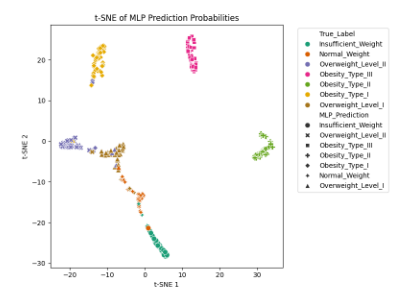
\includegraphics[width=0.45\textwidth]{fig11.png}
\caption{shows the t-SNE of MLP prediction probabilities.}
\label{Table 3.1}
\end{figure}

Similarly, t-Distributed Stochastic Neighbor Embedding (t-SNE) shown in Figure 11 was also applied to the class probabilities to capture nonlinear relationships. It is better suited than PCA for capturing complex patterns in prediction confidence. The clusters were more distinct and organically shaped than those produced by PCA. Obesity\_Type\_I, Obesity\_Type\_II, and Obesity\_Type\_III are the most prominent clusters shown in Figure 11. Insufficient\_Weight forms its own cluster. Normal\_Weight and Overweight levels show some overlap which indicates that the classes in these categories may share similar features which the model finds harder to classify. Despite this, there is still a clear level of separation between the classes which provides clearer insight into instances that were confidently classified and those that were borderline or misclassified. These visualizations confirmed that the MLP model produced higher accuracy and more high-confidence predictions.

One of the more insightful metrics we measured was the Brier score, which reflects the quality of the predicted probability distributions [3]. The Brier score is important in healthcare applications, due to the fact that wrong predictions can have major consequences. Our results showed that the MLP model had much lower Brier scores across the board compared to the Perceptron, with the best performance occurring when using the Top 15 Attributes, producing a Brier score of 0.1096 on the test set. This low Brier score indicates strong classification performance and supports the claim that the Multilayer Perceptron produces well-calibrated probability estimates that avoid overfitting. This is in contrast to the Perceptron which consistently had higher Brier scores, performing poorly in classification. These results demonstrate the Multilayer Perceptron’s suitability for real-world obesity predictions tasks, where the reliability of outputs are paramount.


\section{Related Work}
Presently, several studies have explored the use of machine learning techniques in various fields and subjects in medicine, including predicting obesity and analyzing health-related behaviors. For example, a research paper written by several authors including F.H Yagin (2023) titled, Estimation of Obesity Levels with a Trained Neural Network Approach optimized by the Bayesian Technique, utilized a trained neural network approach optimized by the Bayesian technique to estimate obesity levels, demonstrating that non-linear classifiers like Artificial Neural Networks (ANNs) are highly effective in identifying complex relationships between lifestyle habits and weight categories. Other works have used logistic regression, decision trees, and support vector machines on similar datasets, achieving moderate success but often lacking the ability to handle non-linear decision boundaries as efficiently as ANNs.

The same dataset we used has also been employed in previous studies, such as the paper, Dataset for estimation of obesity levels based on eating habits and physical condition in individuals from Colombia, Peru and Mexico, written by Palechor and Manotas, whose primary goal was to focus on identifying obesity risk based on physical and eating habits in Latin American populations. Though similar, our project additionally incorporates a multi-layer perceptron (MLP) to perform multi-class classification across a broader scope of obesity attributes. In addition, many existing obesity models rely solely on BMI or other simplified features which, as we have seen in our earlier results, do not always yield greater accuracy. In contrast, our model incorporates a wider range of lifestyle attributes, such as those mentioned in Section 3. In terms of performance evaluation, our model leverages the F1-score and Brier score in addition to accuracy whereas much of the current research only utilizes the latter. This offers more insight into classification performance and probability calibration.

We see other researchers try this approach and even exclude height and weight as contributing attributes all together. In a recent study conducted in 2025 by Genc and Arıcan titled Obesity classification: a comparative study of machine learning models excluding weight and height data, an investigation on finding the effectiveness of various machine learning models in classifying obesity levels without relying on height and weight data was conducted using, again, the same dataset we used. They evaluated models such as Random Forest, SVM, Logistic Regression, Neural Networks, and many others. In the end, their results yielded several models with accuracies that still resulted fairly high. Though not as accurate as their counterparts that utilized height and weight, this work highlights the potential of behavioral and demographic data alone to classify obesity levels, supporting our project’s aim of using comprehensive lifestyle features in obesity prediction. 

\section{Conclusion}
Through our research, we were able to showcase that the Multilayer Perceptron consistently outperforms the Perceptron classifier across all metrics. The Multilayer Perceptron’s ability to model nonlinear decision boundaries makes it more effective at capturing the complex relationships in the obesity dataset. In contrast, the Perceptron, being a linear model, struggled with class overlap and frequently misclassified the different categories. This gap in ability was most evident when comparing the confusion matrices and F1-scores, where the Multilayer Perceptron maintained high precision and recall across all classes, even in imbalanced settings. By incorporating behavioral and demographic data, our artificial neural network was able to classify individuals across different levels of obesity with a high degree of accuracy and reliability. This solves the problem of oversimplified diagnosis by providing a model that captures the complexity and diversity of individual health behaviors and how it can contribute to an obesity diagnosis.


\begin{thebibliography}{00}

\bibitem{b1} F. M. Palechor and A. D. L. Hoz Manotas, ``Dataset for estimation of obesity levels based on eating habits and physical condition in individuals from Colombia, Peru and Mexico,'' \textit{Data in Brief}. [Online]. Available: \url{https://www.sciencedirect.com/science/article/pii/S2352340919306985}. [Accessed: Apr. 11, 2025].

\bibitem{b2} S. Adeniran, ``Obesity Prediction Dataset,'' \textit{Kaggle}. [Online]. Available: \url{https://www.kaggle.com/datasets/adeniranstephen/obesity-prediction-dataset}. [Accessed: Apr. 11, 2025].

\bibitem{b3} F. H. Yagin \textit{et al.}, ``Estimation of Obesity Levels with a Trained Neural Network Approach optimized by the Bayesian Technique,'' \textit{Applied Sciences}, vol. 13, no. 6, p. 3875, Jan. 2023, doi: \url{https://doi.org/10.3390/app13063875}.

\bibitem{b4} Comment \textit{et al.}, ``Implementing PCA in python with scikit-learn,'' \textit{GeeksforGeeks}. [Online]. Available: \url{https://www.geeksforgeeks.org/implementing-pca-in-python-with-scikit-learn/}. [Accessed: May 1, 2025].

\bibitem{b5} ``Adding attributes to role-based access control,'' \textit{NIST}. [Online]. Available: \url{https://csrc.nist.gov/files/pubs/journal/2010/06/adding-attributes-to-rolebased-access-control/final/docs/kuhn-coyne-weil-10.pdf}. [Accessed: May 1, 2025].

\bibitem{b6} A. C. Genc and E. Arıcan, ``Obesity classification: A Comparative Study of machine learning models excluding weight and height data,'' \textit{Revista da Associacao Medica Brasileira (1992)}. [Online]. Available: \url{https://pmc.ncbi.nlm.nih.gov/articles/PMC11918863/}. [Accessed: May 2, 2025].
\end{thebibliography}
\section*{Supplementary Material}

The full implementation code and project repository are available on GitHub: 

\begin{itemize}
    \item CS-4210-FinalProject, ``CS-4210-finalproject/final\_project,'' \textit{GitHub}. [Online]. Available: \url{https://github.com/CS-4210-FinalProject/final_project}..
\end{itemize}





\end{document}
